\subsection{I-priors}

\begin{frame}{The regression model}
  \vspace{-5pt}
  \begin{itemize}\setlength\itemsep{1em}
    \item For $i = 1, \dots, n$, consider the regression model
    \begin{align}
      \begin{gathered}
        y_i = f(x_i) + \epsilon_i \\
        (\epsilon_1, \dots, \epsilon_n) \sim \N(\bzero, \bPsi^{-1})
      \end{gathered}
    \end{align}
    where $f \in \cF$, $y_i \in \bbR$, and $x_i = (x_{i1}, \dots, x_{ip}) \in \cX$.
  \end{itemize}
  \begin{center}
    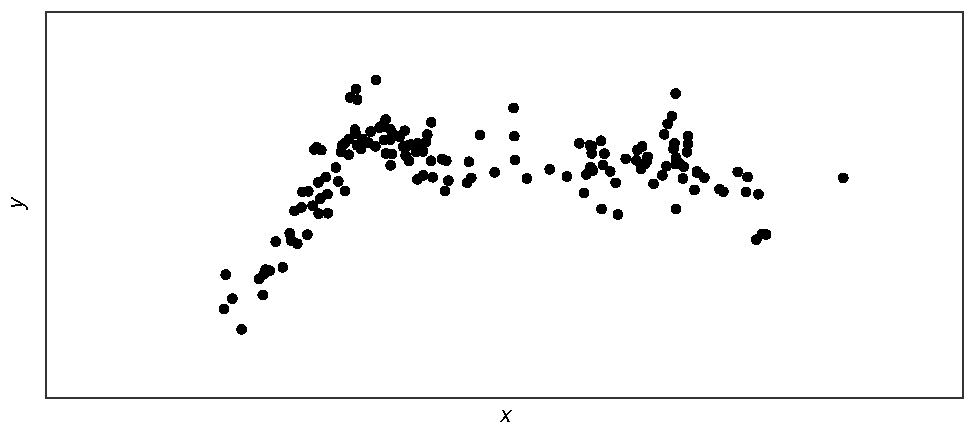
\includegraphics[scale=0.7]{figure/points}
  \end{center}
\end{frame}

\begin{frame}{I-priors}
  \vspace{-16pt}
  \blfootnote{\fullcite{Bergsma2017}}  
  \begin{itemize}\setlength\itemsep{0.3em}
    \item Let $\cF$ be a reproducing kernel Hilbert space (RKHS) with reproducing kernel $h_\lambda: \cX \times \cX \rightarrow \bbR$. An I-prior on $f$ is
    \[
      \big(f(x_1), \dots, f(x_n)\big)^\top \sim \N\big(\bff_0, \cI(f)\big)
    \] 
    with $\bff_0$ a prior mean, and $\cI$ the Fisher information for $f$, given by
    \[
      \cI\big(f(x), f(x')\big) = \sum_{k=1}^n\sum_{l=1}^n \psi_{kl} h_\lambda(x,x_k) h_\lambda(x',x_l).
    \]
    \pause
    \item The I-prior regression model for $i = 1,\dots,n$ becomes
    \begin{align*}
      \begin{gathered}
        y_i = f_0(x_i) + \sum_{k=1}^n h_\lambda(x_i, x_k)w_k + \epsilon_i \\
        (w_1, \dots, w_n) \sim \N(\bzero, \bPsi) \\
        (\epsilon_1, \dots, \epsilon_n) \sim \N(\bzero, \bPsi^{-1})
      \end{gathered}    
    \end{align*}
  \end{itemize}
  \vspace{2pt}
\end{frame}

\begin{frame}{I-priors (cont.)}
  \blfootnote{\fullcite{Jamil2017}}  
  \vspace{-5pt}
  \begin{itemize}\setlength\itemsep{0.8em}
    \item Of interest is the posterior regression function characterised by the distribution
    \[
      p(\bff | \by ) = \frac{p(\by | \bff) p(\bff)}{\int p(\by | \bff) p(\bff) \d\bff} \pause,
    \]
    and also the posterior predictive distribution for new data points $x_{\text{new}}$
    \[
      p(y_{\text{new}} | \by) = \int p(y_{\text{new}} | \by, f_{\text{new}}) p(f_{\text{new}} | \by ) \d f_{\text{new}}
    \]
    with $f_{\text{new}} = f(x_{\text{new}})$.
    \pause
    \item Estimation using EM algorithm or direct maximisation of the marginal likelihood $\log p(y)$.
    \item Complete Bayesian estimation also possible.
  \end{itemize}
  \vspace{5pt}
\end{frame}

%\begin{frame}{Canonical/Linear RKHS}
%  \vspace{-5pt}
%  \only<1>{
%    \begin{center}
%      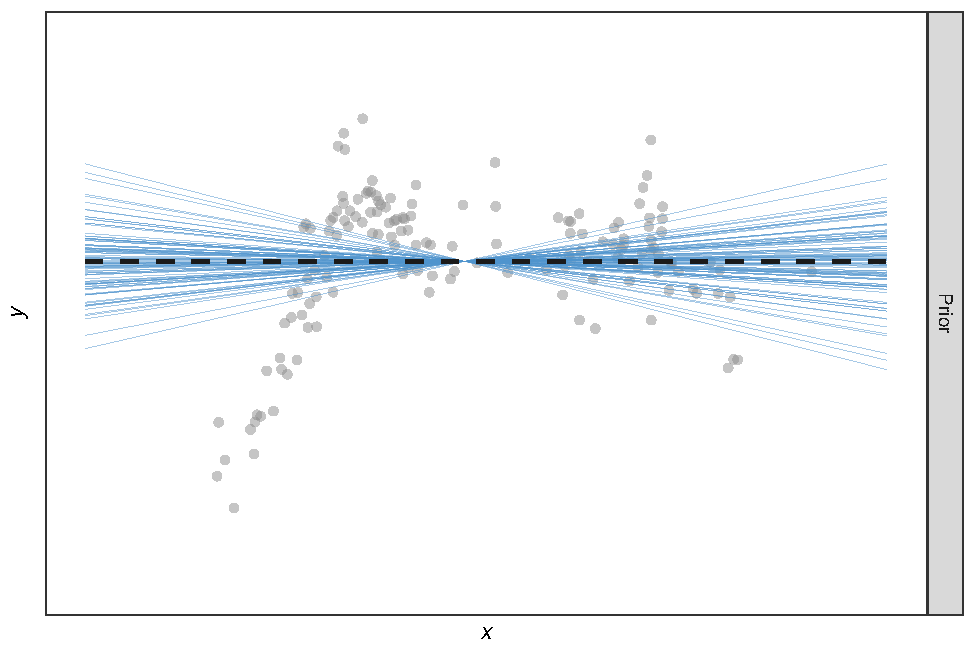
\includegraphics[scale=0.7]{figure/can-prior}
%    \end{center}
%  }
%  \only<2>{
%    \begin{center}
%      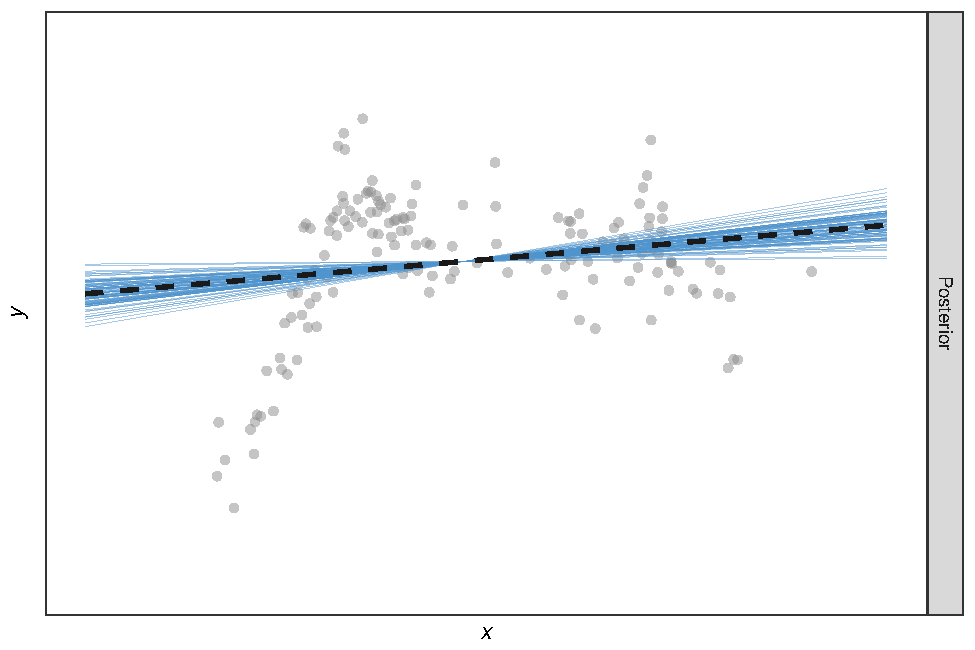
\includegraphics[scale=0.7]{figure/can-posterior}
%    \end{center}
%  }  
%\end{frame}

\begin{frame}{Fractional Brownian motion (FBM) RKHS}
  \vspace{-5pt}
  \only<1|handout:1>{
    \begin{center}
      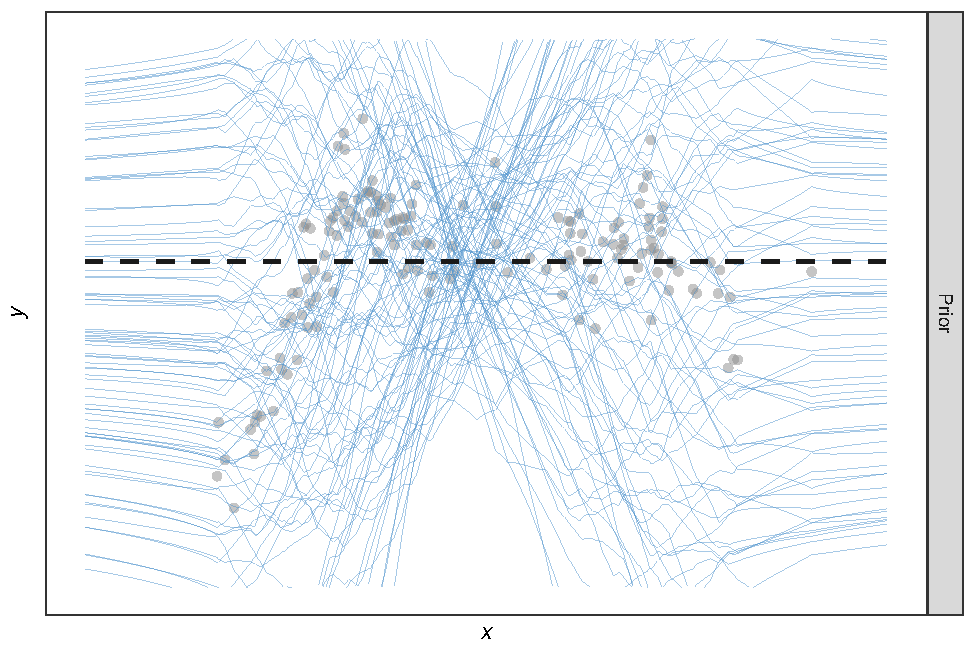
\includegraphics[scale=0.7]{figure/fbm-prior}
    \end{center}
  }
  \only<2|handout:2>{
    \begin{center}
      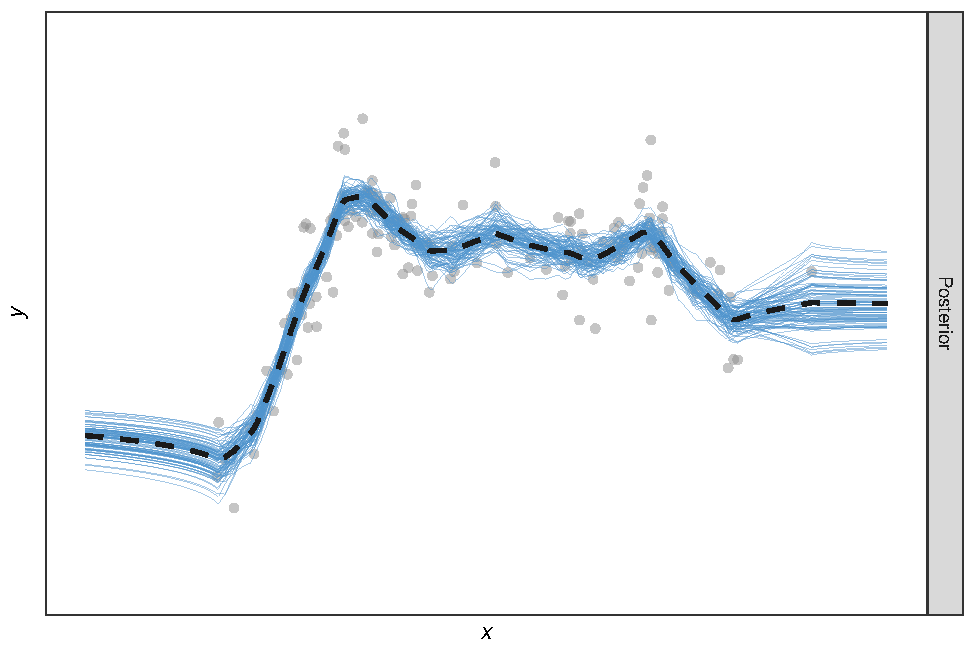
\includegraphics[scale=0.7]{figure/fbm-posterior}
    \end{center}
  }  
  \only<3|handout:3>{
    \begin{center}
      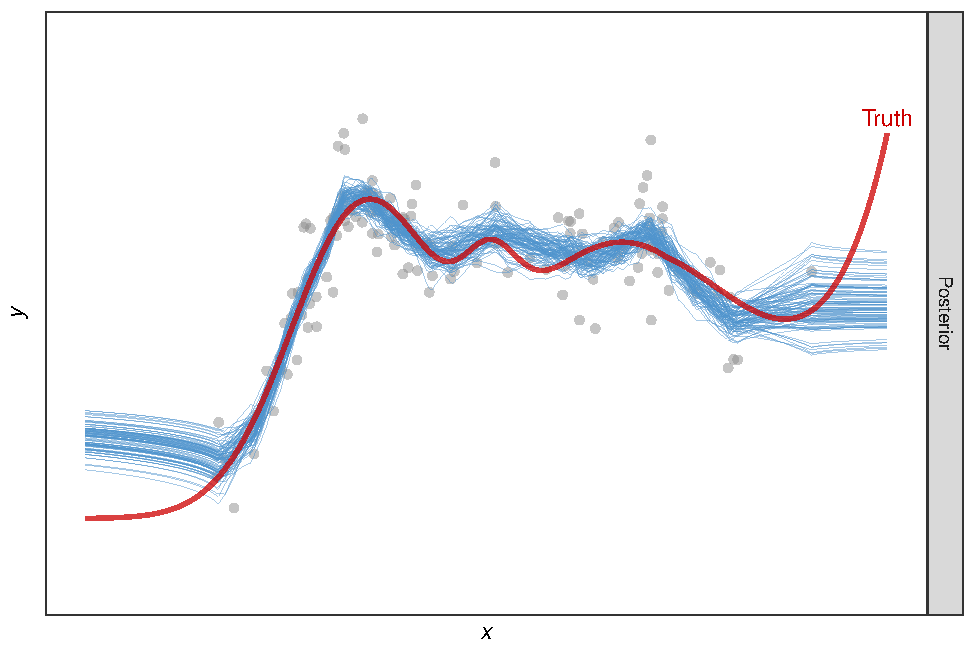
\includegraphics[scale=0.7]{figure/fbm-posterior-truth}
    \end{center}
  } 
\end{frame}

\begin{frame}{Posterior predictive distribution}
  \vspace{-5pt}
  \only<1|handout:1>{
    \begin{center}
      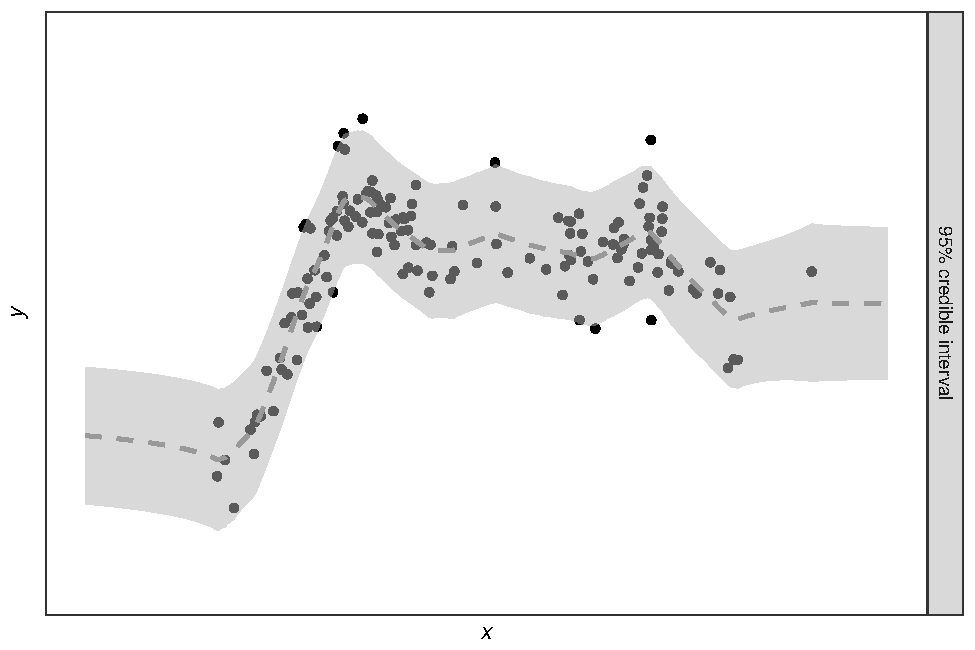
\includegraphics[scale=0.7]{figure/credible-interval}
    \end{center}
  }
  \only<2|handout:2>{
    \begin{center}
      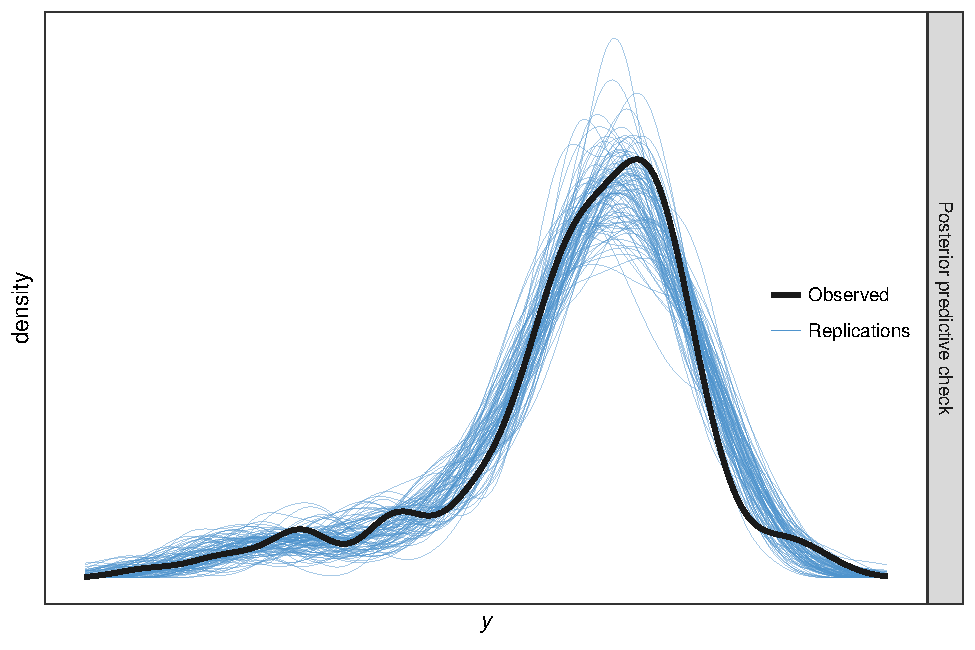
\includegraphics[scale=0.7]{figure/ppc}
    \end{center}
  }
\end{frame}

\subsection{PhD Roadmap}

\begin{frame}{PhD Roadmap}
  \vspace{-28pt}
  \only<1|handout:0>{
    \begin{center}
      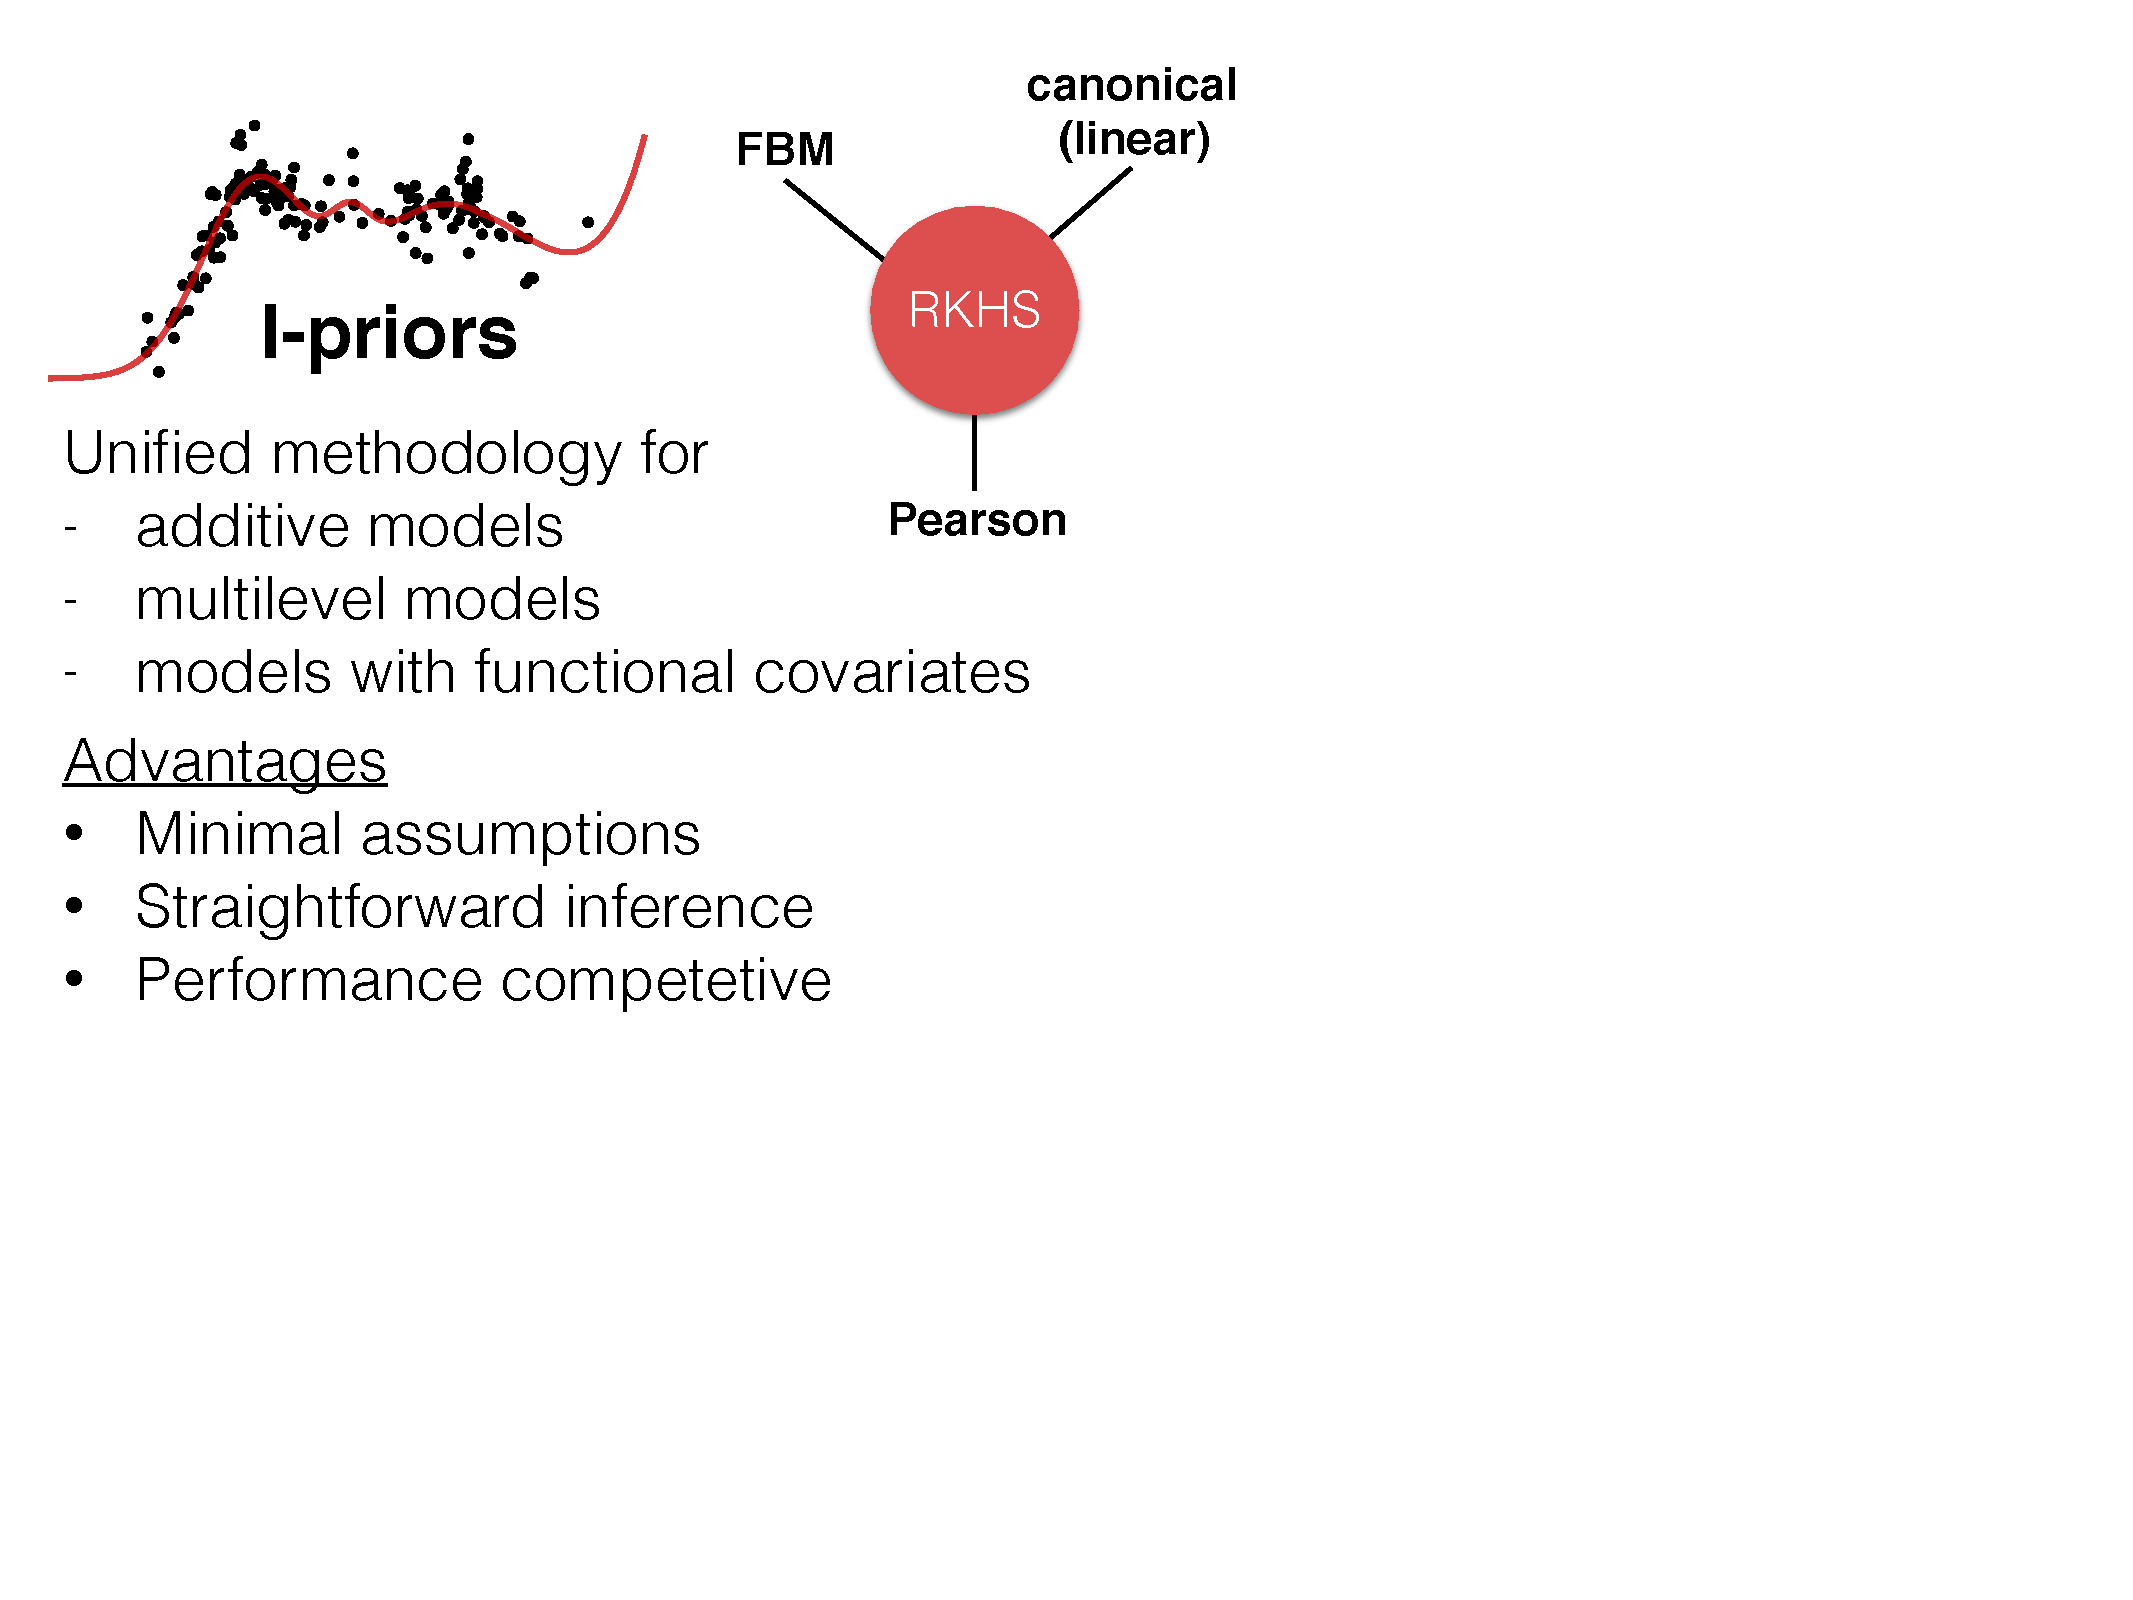
\includegraphics[page=1,width=\textwidth,height=\textheight]{phd-roadmap}
    \end{center}
  }
  \only<2|handout:0>{
    \begin{center}
      \includegraphics[page=2,width=\textwidth,height=\textheight]{phd-roadmap}
    \end{center}
  }  
  \only<3|handout:0>{
    \begin{center}
      \includegraphics[page=3,width=\textwidth,height=\textheight]{phd-roadmap}
    \end{center}
  } 
  \only<4>{
    \begin{center}
      \includegraphics[page=4,width=\textwidth,height=\textheight]{phd-roadmap}
    \end{center}
  } 
\end{frame}





